\section{Zagadnienie brzegowe Dirichleta}
\subsection{Definicja}

Warunek brzegowy Dirichleta stosujemy w teorii równań różniczkowych zwyczajnych oraz cząstkowych (typu eliptycznego) II rzędu.

Polega ona na zalożeniu, że znane są wartości poszukiwanego rozwiązania na obu brzegach przedziału $[a,b]$, na którym określona jest funkcja będąca rozwiązaniem danego problemu.

Jeżeli dla równania różniczkowego (zwyczajnego lub cząstkowego) stawiamy warunek brzegowy Dirichleta (na całym brzegu), to mówimy o zagadnieniu (problemie) Dirichleta. 

\textbf{Warunek brzegowy Dirichleta (I rodzaju)}

\[
\begin{cases}
\vspace{0.1cm} 
\hspace{0,1cm}\alpha \cdot y'' + \beta \cdot y'+\gamma \cdot y=f \\
\vspace{0.1cm}
\hspace{0,1cm}y(a)=y_{a} \\
\hspace{0,1cm}y(b)=y_{b}
\end{cases}
\]
, gdzie:

$\alpha, \beta, \gamma, f$ są znanymi funkcjami
\newline
$y = y(x)$ jest poszukiwanym rozwiązaniem
\newline

\textbf{Zagadnienie Dirichleta}

Poszukujemy funckję $u$, której znane są wartości na brzegu. Taki problem da się rozwiązać analitycznie całkując dwukrotnie równanie.

\[
\begin{cases}
\vspace{0.1cm} 
\hspace{0,1cm}u''=f \\
\vspace{0.1cm}
\hspace{0,1cm}u|_{x=a}=u_{a} \\
\hspace{0,1cm}u|_{x=b}=u_{b}
\end{cases}
\]
\newline

My jednak sformułujemy to zagadnienie z użyciem MRS, otrzymamy wówczas aproksymację rozwiązania w wybranych przez nas węzłach.

Następnie porównamy metodę numeryczną oraz analityczną rozwiązania zadanego problemu.

\subsection{Cel ćwiczenia}

Naszym zadaniem było stworzenie algorytmu rozwiązującego następujące zagadnienia Dirichleta:

a)
\[
\begin{cases}
\vspace{0.1cm} 
\hspace{0,1cm}u''=-sin(x)-4\cdot sin(2x) \\
\vspace{0.1cm}
\hspace{0,1cm}u|_{x=0}=0 \\
\hspace{0,1cm}u|_{x=2\pi}=0
\end{cases}
\]
, gdzie:

$x\in [0,2\pi]$

Rozwiązanie analityczne: $\widetilde{u}(x) = sin(x) +sin(2x)$
\newpage
b)
\[
\begin{cases}
\vspace{0.1cm} 
\hspace{0,1cm}u''=12x \\
\vspace{0.1cm}
\hspace{0,1cm}u|_{x=0}=0 \\
\hspace{0,1cm}u|_{x=1}=1
\end{cases}
\]
, gdzie:

$x\in [0,1]$

Rozwiązanie analityczne: $\widetilde{u}(x) = 2x^{3}-x$

\vspace{0.3cm}
Ponadto zaprezentujemy wykres porównujący rozwiązanie numeryczne z rozwiązaniem analitycznym, a także wykres błędu $||E||_{\infty}$ w zależności od liczby obranych węzłów (n).

\subsection{Algorytm}
a)
\begin{samepage}
\begin{Shaded}
\begin{Highlighting}[]
\FunctionTok{clear}\NormalTok{, }\FunctionTok{clc}\NormalTok{;}
\CommentTok{#dane wejściowe}
\NormalTok{a=}\FloatTok{0}\NormalTok{;}
\NormalTok{b=}\FloatTok{2}\NormalTok{*}\BaseNTok{pi}\NormalTok{;}
\NormalTok{n = input('Podaj liczbe węzłów: ');}
\NormalTok{h = (b-a)/(n-}\FloatTok{1}\NormalTok{);}
\NormalTok{Ua = }\FloatTok{0}\NormalTok{;}
\NormalTok{Ub = }\FloatTok{0}\NormalTok{;}
\NormalTok{f = @(x) -}\FunctionTok{sin}\NormalTok{(x) - }\FloatTok{4}\NormalTok{*}\FunctionTok{sin}\NormalTok{(}\FloatTok{2}\NormalTok{*x);}
\NormalTok{g = @(x) }\FunctionTok{sin}\NormalTok{(x) + }\FunctionTok{sin}\NormalTok{(}\FloatTok{2}\NormalTok{*x);}
\CommentTok{#obliczenia}
\NormalTok{v1 = -}\FloatTok{2}\NormalTok{*}\FunctionTok{diag}\NormalTok{(}\FunctionTok{eye}\NormalTok{(n));}
\NormalTok{v2 = }\FunctionTok{diag}\NormalTok{(}\FunctionTok{eye}\NormalTok{(n-}\FloatTok{1}\NormalTok{));}
\NormalTok{A = }\FunctionTok{diag}\NormalTok{(v1) + }\FunctionTok{diag}\NormalTok{(v2,}\FloatTok{1}\NormalTok{) + }\FunctionTok{diag}\NormalTok{(v2,-}\FloatTok{1}\NormalTok{);}
\NormalTok{x= }\FunctionTok{linspace}\NormalTok{(a+h,b-h,n);}
\NormalTok{x2 = }\FunctionTok{linspace}\NormalTok{(a,b,n+}\FloatTok{2}\NormalTok{);}
\NormalTok{x3 = }\FunctionTok{linspace}\NormalTok{(a,b,100}\NormalTok{);}
\NormalTok{F = f(x)*h^}\FloatTok{2}\NormalTok{;}
\NormalTok{F(}\FloatTok{1}\NormalTok{) = F(}\FloatTok{1}\NormalTok{) - Ua;}
\NormalTok{F(n) = F(n) - Ub;}
\NormalTok{U = linsolve(A,F');}
\NormalTok{U = [Ua U' Ub];}
\CommentTok{#wykres}
\NormalTok{plot(x3, g(x3), x2, g(x2), 'ro');}
\NormalTok{legend('Metoda Analityczna','Metoda Numeryczna');}
\CommentTok{#error}
\NormalTok{E = max(abs(g(x2) - U));}
\end{Highlighting}
\end{Shaded}
\end{samepage}
\newpage
b)
\begin{samepage}
\begin{Shaded}
\begin{Highlighting}[]
\FunctionTok{clear}\NormalTok{, }\FunctionTok{clc}\NormalTok{;}
\CommentTok{#dane wejściowe}
\NormalTok{a=}\FloatTok{0}\NormalTok{;}
\NormalTok{b=}\FloatTok{1}\NormalTok{;}
\CommentTok{#n=input('Podaj liczbę węzłów: ');}
\NormalTok{n = }\FloatTok{10}\NormalTok{;}
\NormalTok{h = (b-a)/(n-}\FloatTok{1}\NormalTok{);}
\NormalTok{Ua = }\FloatTok{0}\NormalTok{;}
\NormalTok{Ub = }\FloatTok{1}\NormalTok{;}
\NormalTok{f = @(x) }\FloatTok{12}\NormalTok{*x;}
\NormalTok{g = @(x) }\FloatTok{2}\NormalTok{*x.^}\FloatTok{3}\NormalTok{-x;}
\CommentTok{#obliczenia}
\NormalTok{v1 = -}\FloatTok{2}\NormalTok{*}\FunctionTok{diag}\NormalTok{(}\FunctionTok{eye}\NormalTok{(n));}
\NormalTok{v2 = }\FunctionTok{diag}\NormalTok{(}\FunctionTok{eye}\NormalTok{(n-}\FloatTok{1}\NormalTok{));}
\NormalTok{A = }\FunctionTok{diag}\NormalTok{(v1) + }\FunctionTok{diag}\NormalTok{(v2,}\FloatTok{1}\NormalTok{) + }\FunctionTok{diag}\NormalTok{(v2,-}\FloatTok{1}\NormalTok{);}
\NormalTok{x= }\FunctionTok{linspace}\NormalTok{(a+h,b-h,n);}
\NormalTok{x2 = }\FunctionTok{linspace}\NormalTok{(a,b,n+}\FloatTok{2}\NormalTok{);}
\NormalTok{x3 = }\FunctionTok{linspace}\NormalTok{(a,b,100}\NormalTok{);}
\NormalTok{F = f(x)*h^}\FloatTok{2}\NormalTok{;}
\NormalTok{F(}\FloatTok{1}\NormalTok{) = F(}\FloatTok{1}\NormalTok{) - Ua;}
\NormalTok{F(n) = F(n) - Ub;}
\NormalTok{U = linsolve(A,F');}
\NormalTok{U = [Ua U' Ub];}
\CommentTok{#wykres}
\NormalTok{plot(x3, g(x3), x2, g(x2), 'ro');}
\NormalTok{legend('Metoda Analityczna','Metoda Numeryczna',0);}
\CommentTok{#error}
\NormalTok{E = max(abs(g(x2) - U));}

\end{Highlighting}
\end{Shaded}
\end{samepage}
\newpage
\subsection{Wykresy}
a)

Dla 10 węzłów:

\begin{figure}[!ht]
	\begin{center}
		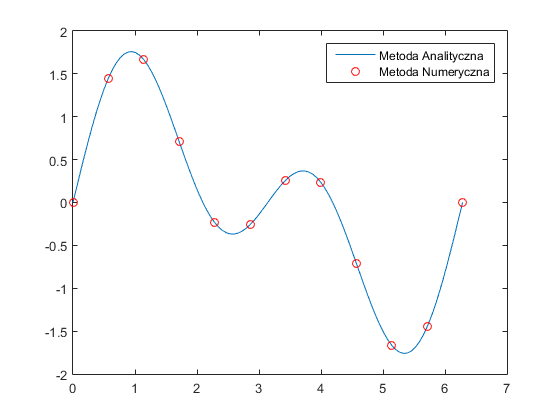
\includegraphics[width=0.8\textwidth]{Lab3/charts/zad1/10.png}
	\end{center}
\end{figure}

Dla 25 węzłów:

\begin{figure}[!ht]
	\begin{center}
		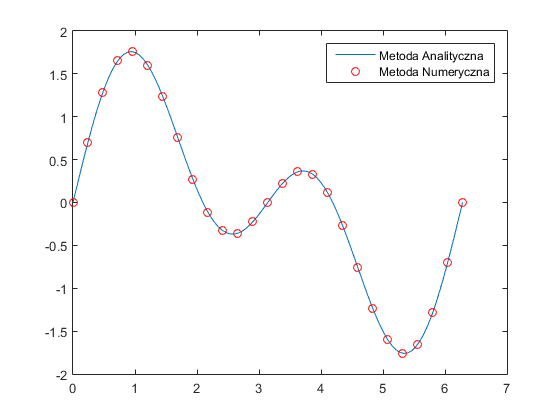
\includegraphics[width=0.8\textwidth]{Lab3/charts/zad1/25.png}
	\end{center}
\end{figure}

\newpage

Dla 100 węzłów:
	

\begin{figure}[!ht]
	\begin{center}
		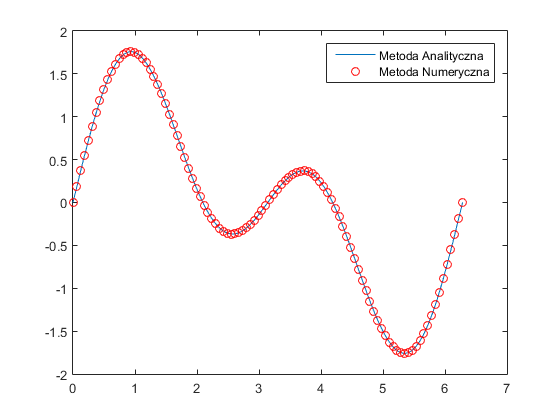
\includegraphics[width=0.8\textwidth]{Lab3/charts/zad1/100.png}
	\end{center}
\end{figure}



Dla 1000 węzłów:

\begin{figure}[!ht]
	\begin{center}
		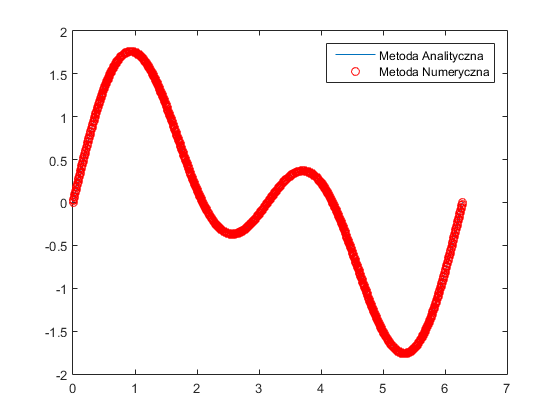
\includegraphics[width=0.8\textwidth]{Lab3/charts/zad1/1000.png}
	\end{center}
\end{figure}

\newpage

Błąd metody w zależności od liczby węzłów:

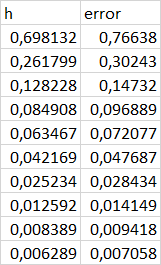
\includegraphics{Lab3/charts/zad1/error_dane.png}

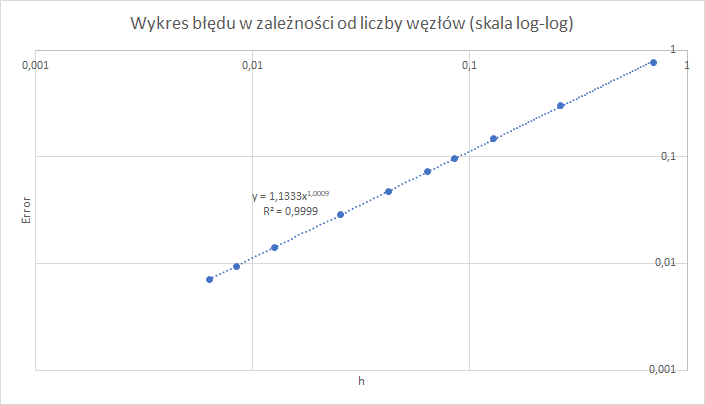
\includegraphics{Lab3/charts/zad1/error.png}

\newpage

b)

Dla 10 węzłów:

\begin{figure}[!ht]
	\begin{center}
		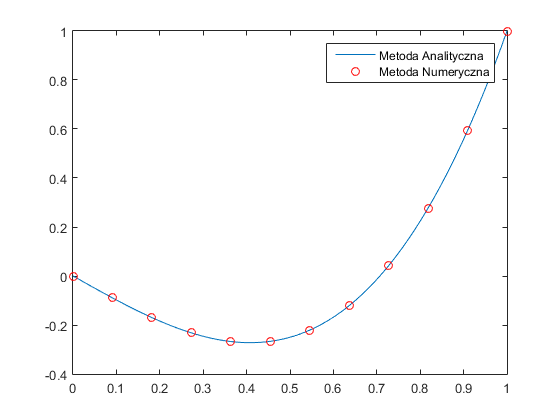
\includegraphics[width=0.8\textwidth]{Lab3/charts/zad2/10.png}
	\end{center}
\end{figure}

Dla 25 węzłów:

\begin{figure}[!ht]
	\begin{center}
		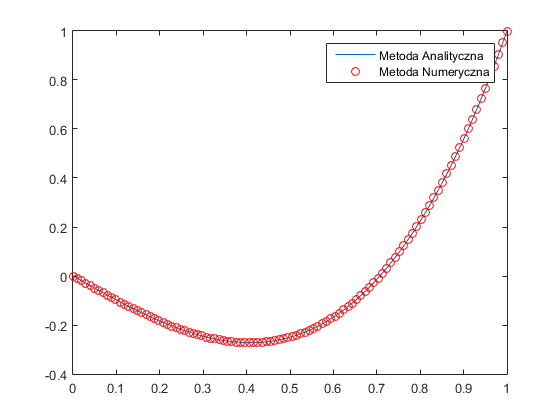
\includegraphics[width=0.8\textwidth]{Lab3/charts/zad2/25.png}
	\end{center}
\end{figure}

\newpage

Dla 100 węzłów:

\begin{figure}[!ht]
	\begin{center}
		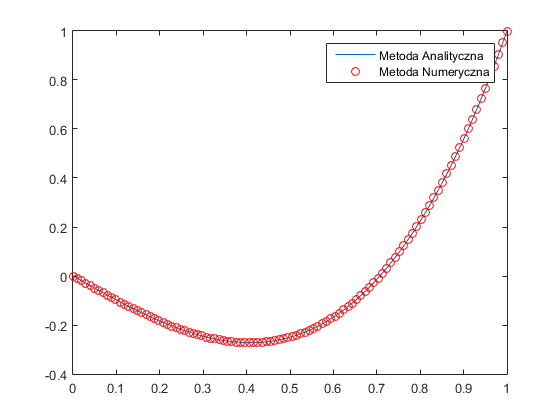
\includegraphics[width=0.8\textwidth]{Lab3/charts/zad2/100.png}
	\end{center}
\end{figure}

Dla 1000 węzłów:

\begin{figure}[!ht]
	\begin{center}
		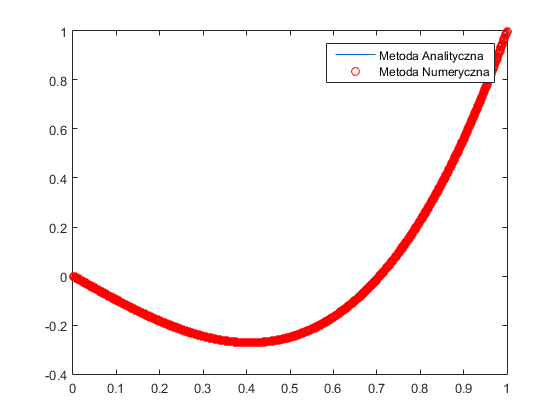
\includegraphics[width=0.8\textwidth]{Lab3/charts/zad2/1000.png}
	\end{center}
\end{figure}

\newpage

Błąd metody w zależności od liczby węzłów:

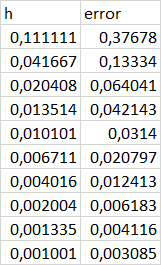
\includegraphics{Lab3/charts/zad2/error_dane.png}

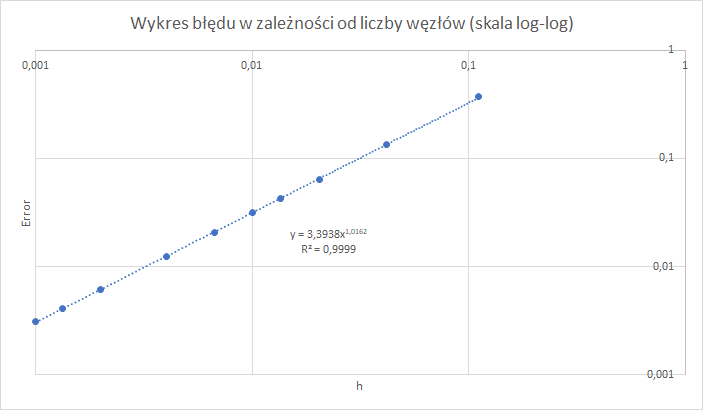
\includegraphics{Lab3/charts/zad2/error.png}

